\begin{figure}[htp] \centering
    \begin{subfigure}[b]{0.96\columnwidth}
        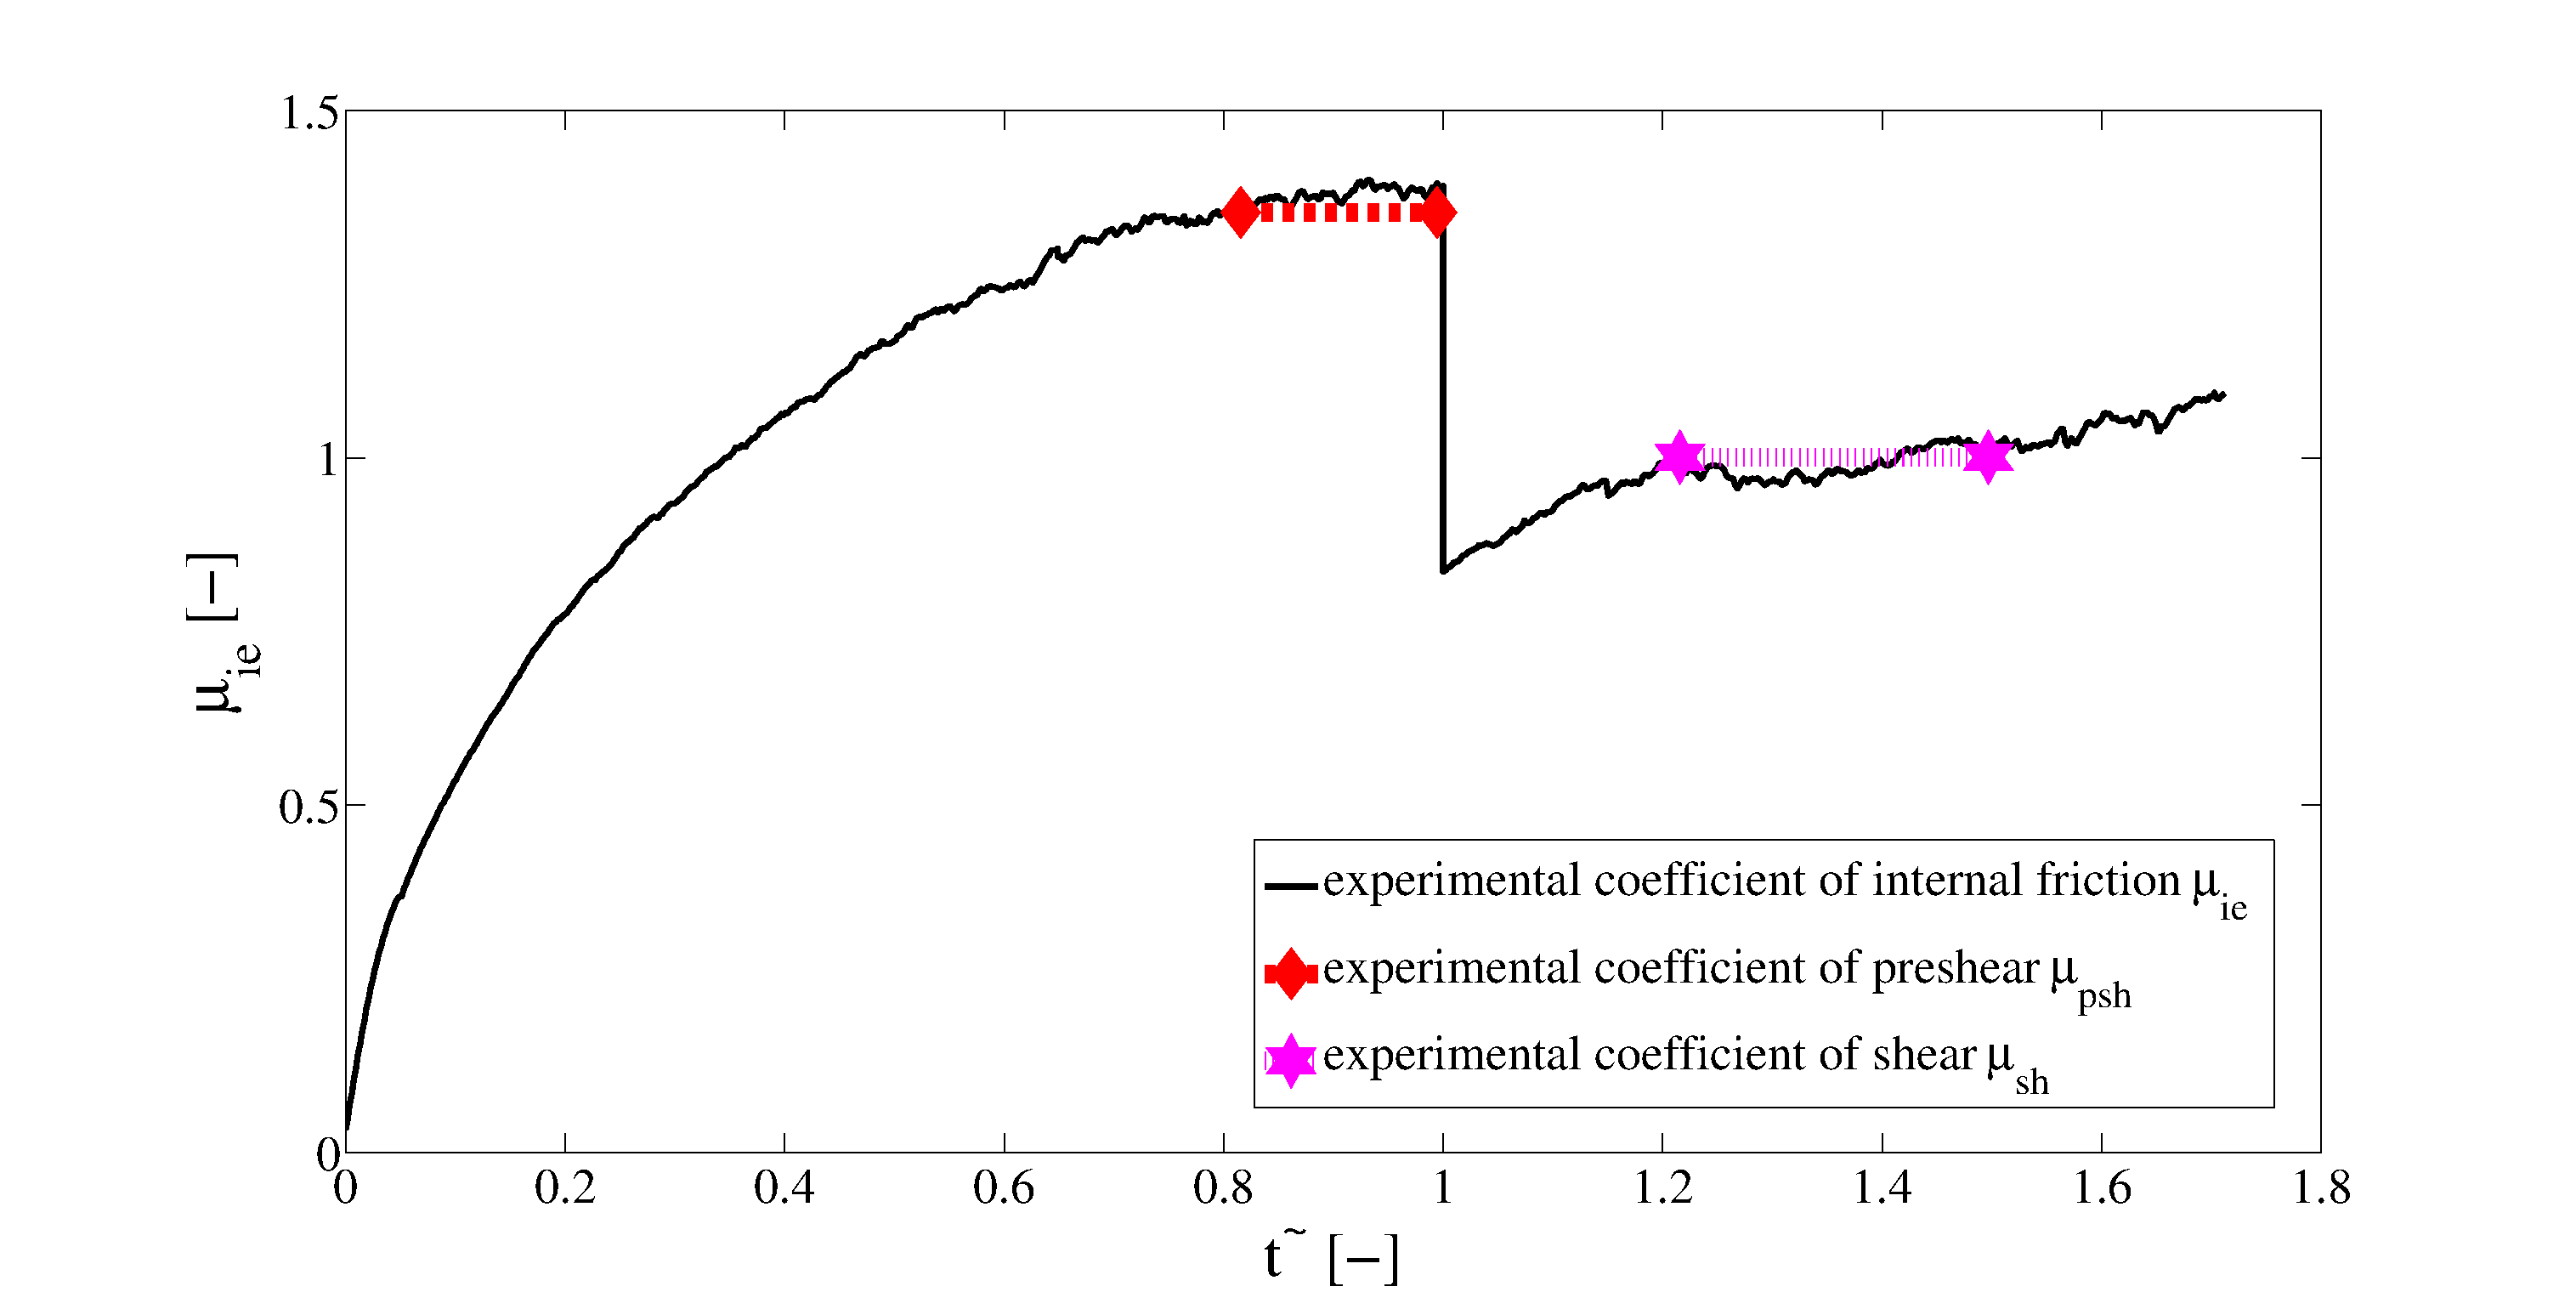
\includegraphics[width=\textwidth]{20experimental}
        \caption{Experimental shear cell tester stress path - $\sigma_n = 10000
        [Pa]$}
        \label{fig:20experimental} 
    \end{subfigure}\\
        \begin{subfigure}[b]{0.96\columnwidth}
        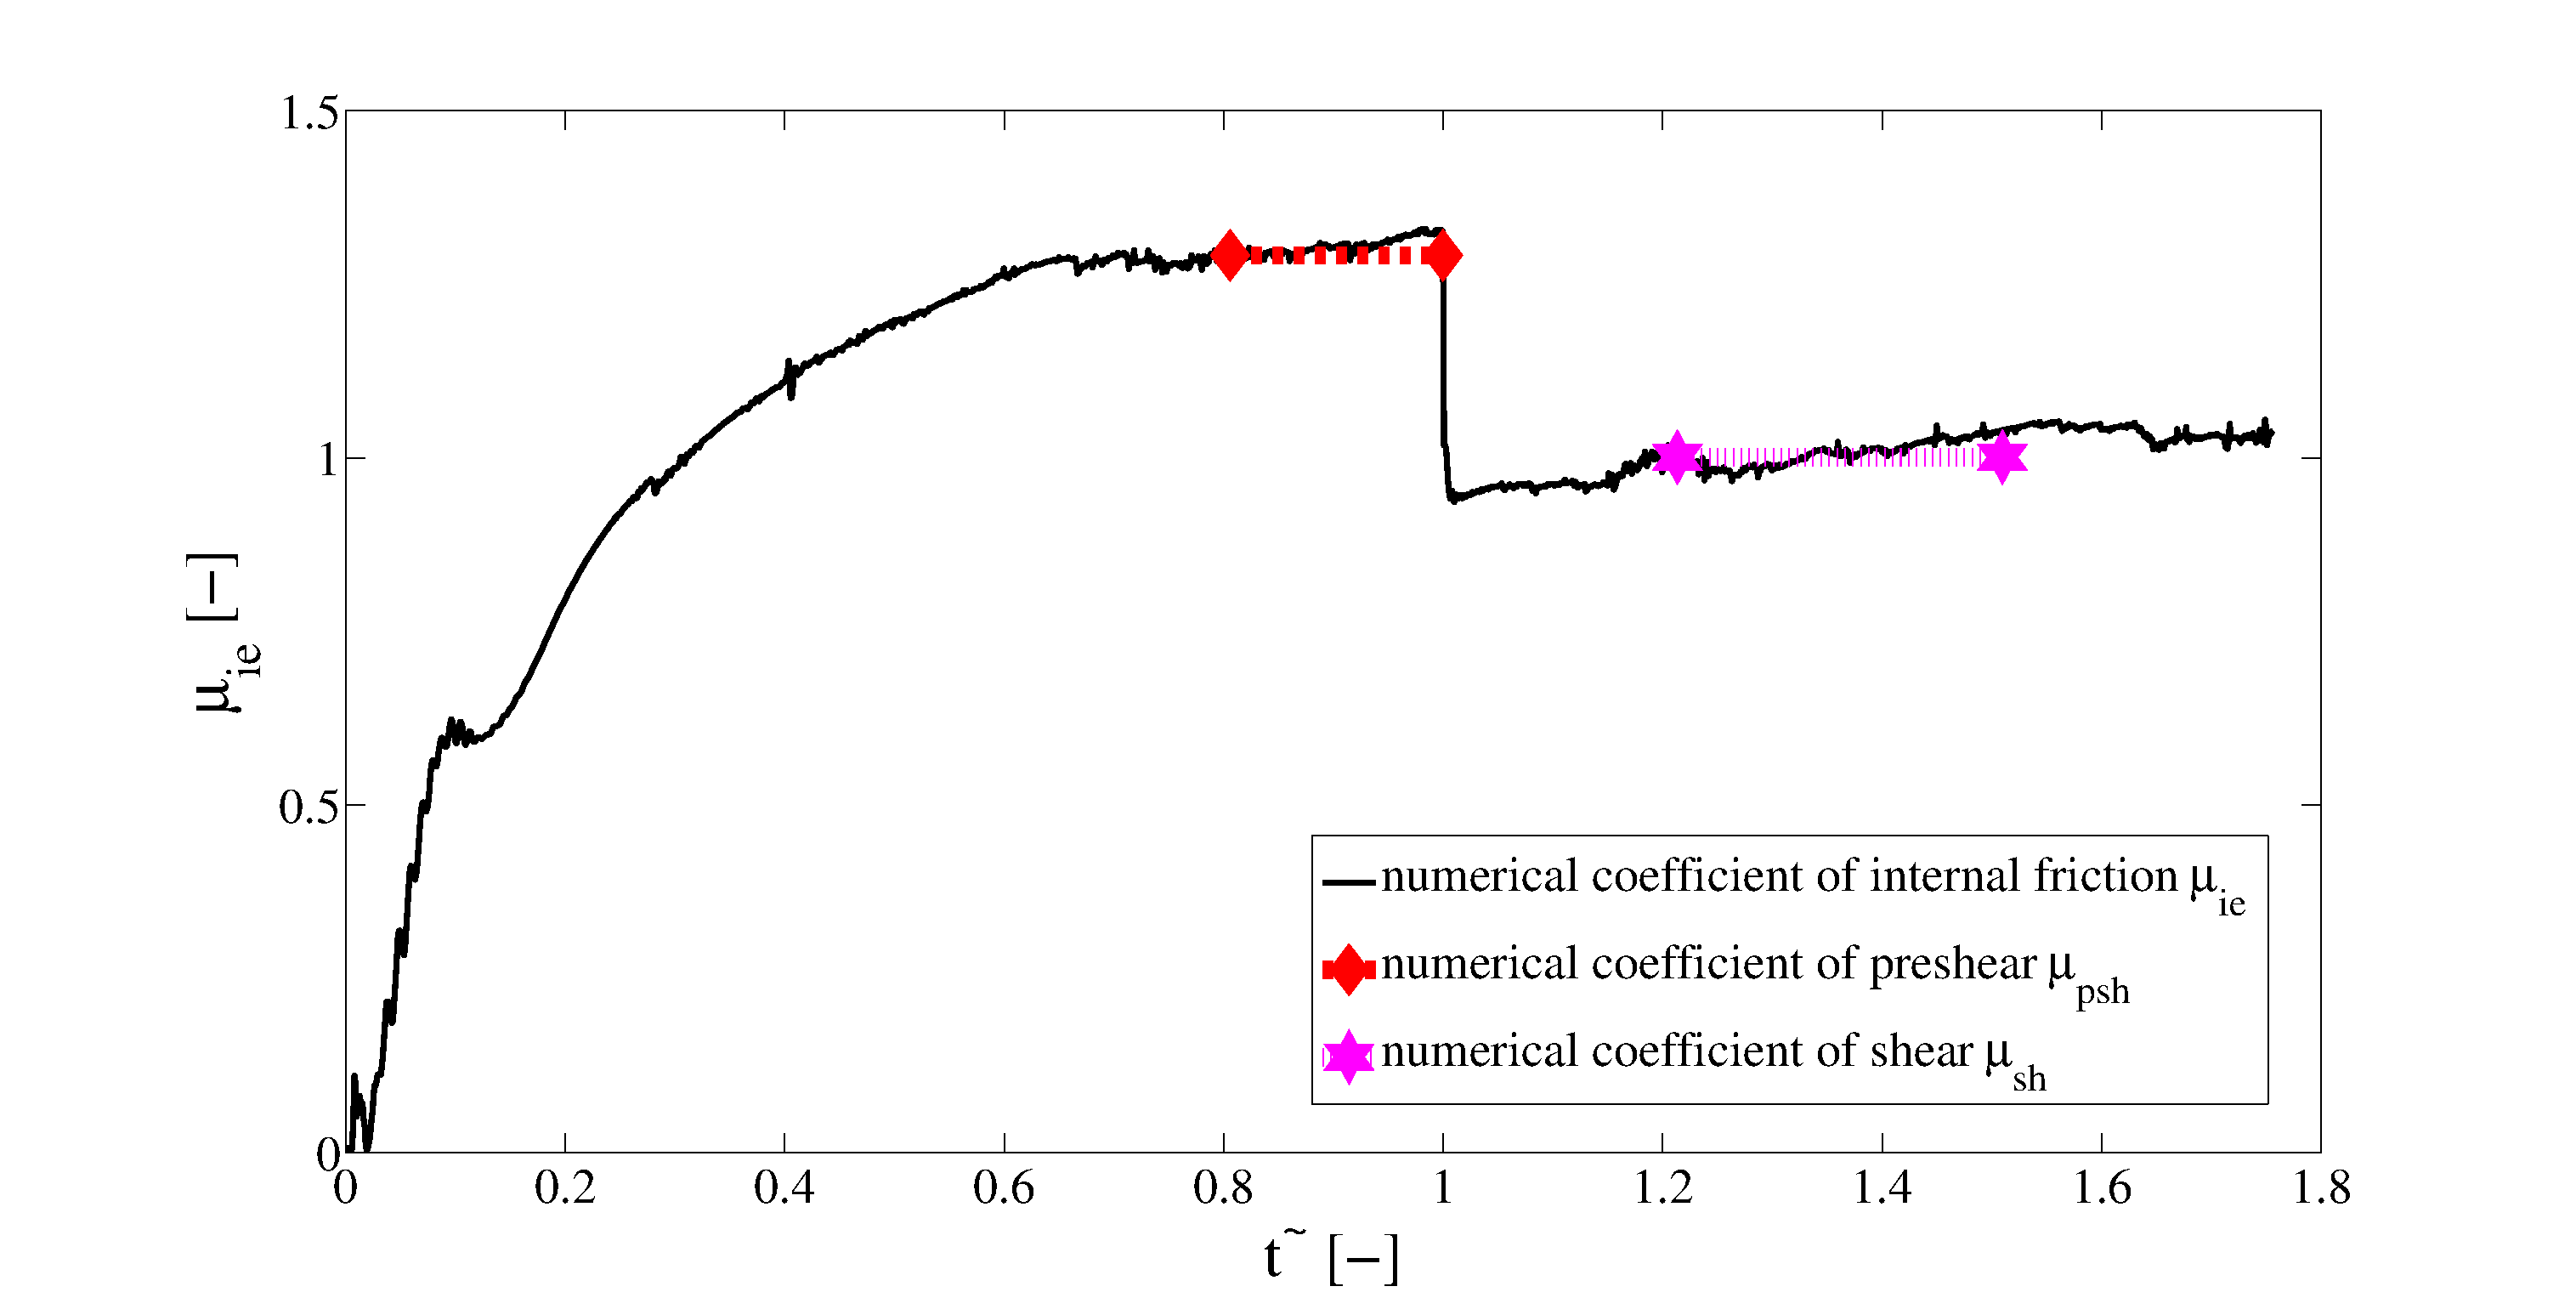
\includegraphics[width=\textwidth]{21simexample}
        \caption{Numerical shear cell tester stress path - $\sigma_n = 10000
        [Pa]$}
        \label{fig:21simexample} 
    \end{subfigure}
    \caption[Stress path]{Sample of the stress path for
	the Schulze ring shear cell tester, experimental and numerical.
	Time is normalized: $\tilde{t} = t/t_{change}$, where $t_{change}$ is the
	time when the normal stress ($\sigma_n$) is modified during the tests.
	Until $\tilde{t}=1$ the $\sigma_n = 10000 ~[Pa]$ is kept constant. 
	In Fig. \ref{fig:20experimental} at $\tilde{t}~=0.91$
 	a plateau is reached.
	The coefficient of pre-shear ($\mu_{psh}$) is calculated as average of the
	coefficient of internal friction ($\mu_{ie}$) in this first plateau.
	Later, at $\tilde{t}=1$, the $\sigma_n$ is reduced to $80 \%$ of its initial
	value.
	Soon, a second plateau starts.
	As average of $\mu_{ie}$ in this second plateau we obtain coefficient of
	shear ($ \mu_{sh}$).
	The stress path is in the numerical simulation is comparable to the
	experimental one, especially the plateaux.
	They were clearly relevant because there we collected the numerical bulk
	behaviour representative values. }
    \label{fig:40experimentalsimulation}
\end{figure}
